%!TEX root = project.tex

\chapter*{About this project}
\paragraph{Abstract}
The project that was undertaken is called “Alumni Registration and Linking Application” also known as Arla. What is Arla? It is an application that was originally intended to be developed on behalf of the college itself. The original idea was that GMIT was to use it on their website. Arla is where users can sign up and login to the system, add information to their profile and create connections with other users using the messenger part of the application

\paragraph{Authors}
Ciaran Roche, 4th year student at GMIT, student number G00376934\\

\subsection{Github source code}
\url{https://github.com/CiaranRoche203/Arla-App-FrontEnd}\\
\url{https://github.com/CiaranRoche203/Arla-App-Backend}\\

\subsection{Heroku Hosted Application}
\url{https://arl-application.herokuapp.com/}\\
\chapter{Introduction}

\section{Accessibility}
The application is designed so that it is very user friendly to people of all ages and all experiences of using technology. For example, it was intended to make sure that someone who has never used a computer before in their life has as much ease of using the application as someone who uses it every day. The user will also have as much flexibility as they like when it comes to the information that people are able to access about them on the website. The user may decide they don’t want to have any connections and not upload any information to the application. Perhaps they just want to have a browse on the application without actually connecting to people. 

\section{Why this Project}
It is a good project to develop at level 8 as there is so many different ways the project can be implemented with, given enough time, many cool features can also be implemented. Another reason as to why it was a good project for a final year project is because of the complexity and workload of it. These technologies used were extremely complex and took a lot of research and reading of documentation to fully understand and implement. 

\section{Front End}
The front end of the application was developed using React.\cite{AngularvsReact} The graphical part of the application was implemented using D3.js.\cite{D3.js} There were some new and exciting libraries that were implemented into the application also. These were chatengine.io\cite{Chatengine} and react popup\cite{popup} as well as some libraries that were intended for use but could not properly use for one reason or another. These technologies and libraries will be discussed some more in the technology review section of the document. The application is fully responsive on the front end that can only be accessed if the user has logged in. It is also set up on Heroku so that it can be accessed publicly. Below in the Appendices chapter are links to the application hosted on Heroku along with the GitHub repositories where the work was stored. 

\section{Back End}
The back end had many issues in the development process which will be discussed more in the dissertation and outline the course of action that the supervisors advised to take. The back end connected to the new technology Neo4J\cite{Neo4J} which is a graph-based database where all the information passed from the front end was to be stored. The graph on the React front end was essentially the Neo4J database superimposed using D3. 

\section{Goals and Objectives}
There were many goals set at the beginning of the project before development initially took place, and it was hoped that as many as possible if not all of them were implemented and completed by the end of the project life cycle. The goals that were set were as follows: 

\begin{itemize}
\item Create a fully responsive web application that is hosted on a middle ware site such as Heroku or AWS that allows for users to connect to each other and message each other via a messenger styled page on the application. 
\item Accommodate all people who wish to use their website, make it extremely simple, efficient and user friendly for both a user with no previous experience of using technology and someone who has high levels of experience in using technology.
\item To allow the user to enter as much or as little detail as they wish and to decide how much of this information would be visible to other users of the application. Along with this, it was also a goal to make sure that the user can adjust or remove any details they may have inadvertently added to their profile.
\item Create a way in which users can create their own groups and contact each other. Perhaps along with this create their own little mini graph and show all the people within the group. They could then have a group chat on the messenger page for example. 
\item Gain a greater understanding of the technologies that were going to be used in development and to learn some new and exciting technologies such as D3 and Neo4J in the process. 
\item Create a google login application and understand the mechanics of what is behind this and understand how to implement this for future projects
\item Have a dynamic home page for the user and understanding how to implement this. In other words, when the user logs in, it should show only their individual details on their home page, so that it would be different for every user of the application.
\item Understand how to draw graphs and essentially understand the basic concepts that were needed for this application using D3
\item It was also preferable to improve any testing skills throughout the duration and at the completion of programming the application. 
\item Improve any ability to use the Jira application and learn how it can be incorporated it into the project. This is so that it improves efficiency when planning and implementing a project during a project life cycle
\item Ideal to incorporate fully and improve usage of OneNote for documentation and GitHub for the programming aspect of the project. 
\item It was ideal and preferable to improve soft skills. Improving any skills such as teamwork and communication by having regular meetings with the supervisor. This is ideal to constantly keep people up to date with the project as well as making sure it is on the right track. 
\end{itemize}

\section{Methodology}
The methodology chapter in this paper is where the projects methodology will be discussed and essentially how the project was carried out and implemented. The development approach that was used will be discussed under topics such as, how it faired and an evaluation of the style that was adopted. As well as this the planning stages of the project will be discussed. An in-depth look will be taken at what technologies that were used in the early days to set a plan out for the project, how this developed as time progressed and how changes were dealt with. A thorough and in depth look at the technologies that were used for documentation, planning and designing of the project. The tools that were used to develop the project will be discussed and analysed, for example, GitHub. The research that was conducted in the planning stages of the project will be thoroughly explained, dissected and analysed. Also, a delve into the weekly meetings and communication throughout the project will take place. 

\section{Technology Review}
The technology review section is where an in-depth look will take place at all the different technologies that were used in the development process of the project. Some of these technologies will include react, D3, chatengine.io and all the different libraries that were either implemented successfully or implemented unsuccessfully for one reason or another. A brief look will be taken as to why said technologies were not implemented and what alternatives can be or were used instead. Each technology will be analysed to the fullest extent. 

\section{System Design}
The system design section is the part in which a detailed explanation of the overall system architecture will be given. This is essentially the HOW of the project. It is where the knowledge gained from research is implemented. Also, it will look at each aspect of the application and give a detailed overview and in-depth analysis of different components of the system and how they work together. 

\section{System Evaluation}
The system evaluation section is where an evaluation of the system is conducted. For example, what is good, what is bad, what needs more work and what could be done to make this even better. An evaluation of goals will be made, where they met, if not why?

\section{Conclusions}
Finally, a conclusion to the project will be given and an overall opinion of how the project went. Analysis will take place to see what can be done to improve the project as well as performances of members. An evaluation will be made on what was learned during the project cycle.

\chapter{Methodology}

There was a lot of planning, research and decision making that went into the early days approach to the project. The first and most important aspect was to set out a stable plan that the team members can follow. The first step in planning that took place before all else was to research heavily and thoroughly. Research is a common practise that took place in the duration of the project. 

\section{Approach}
The first stage of research involved which type of methodology suited the project and the team members best. There was a general idea of which methodology suited the project best before any research was done but it was important that this was done correctly as it would benefit the planning and overall flow of the project. The 2 cycles that were researched were the Waterfall and Agile.\cite{Methodologies}\\ 

After much deliberation and with advice from the supervisor, it was decided that an Agile approach benefitted the project the most. The reason for this is due to Agiles’ flexibility. It also was a preferred methodology to follow as it allowed for consistent testing of the application as well as receiving consistent feedback\cite{Methodologies}. Waterfall could and probably would have caused a lot of issues overall if it were the methodology that was pursued. The reasoning for not taking on the waterfall model is that it is too rigid. In order to move on to the next step, i.e., design to implementation, the design phase must be one hundred per cent complete. \\

It was then decided that Agile would be the development methodology to be followed. Agile allowed for the project to be developed while minimizing risk when adding new functionality. Some of the risks that it minimized were bugs and changing of requirements. The consistency of testing the application that would take place with Agile would cause less issues in the long run and would not delay development as much as waterfall potentially could. The flexibility was a key factor for the choice of Agile. The ability to make continuous changes and additions to the application coupled with the fact that these new additions and changes would be tested consistently immediately after implementation was a major factor in the decision. \\

\section{Planning}

The next stage in the development of the project was to plan. The plan is crucial as it sets a basis of what needs to be done, by when and by who. The plan is a fundamental necessity to this or any project as without one, it will be a disaster so to speak. The first stage of planning was to hold a meeting with the supervisor. In this meeting the overall project was discussed with the objectives and tasks being set out from the beginning. An idea was given as to what the final project should eventually look like. This was used as a guideline, but changes could always be made to add cool new features to the project. The next stage of planning involved designing the system. It was imperative to get an understanding of what would be happening with the application, what sort of data would be passed from front to back end, where it will be stored etc. Following this, some front-end design was drawn up to get a basic understanding of what a final product may look like (see system design diagrams). Discussion between team members and supervisor was had over the potential design and some changes and additions were made accordingly. The final stage of the first phase of planning was to set up a Jira board. On this Jira the following were set up: 

\subsection{Roadmap}
\begin{figure}[h]
    \centering
    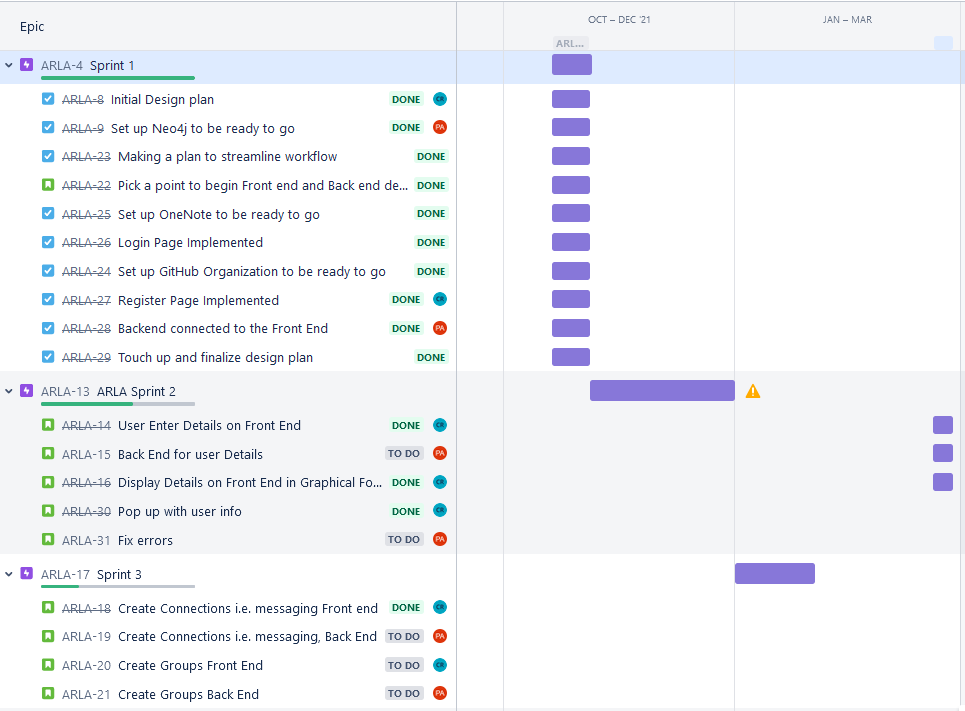
\includegraphics[width=15cm, height=12cm]{img/Roadmap.png}
    \caption{Roadmap}
    \label{fig:my_label}
\end{figure}

The roadmap is a useful tool that allows for a visual representation of the project progress. It is essentially a Gantt chart. The sprints could be adjusted accordingly as needed. For example, if sprint one was taking longer than initially planned, simply moving the bar on the chart allowed for the sprint to continue until the new date it was moved to. 

\subsection{Backlog}
\begin{figure}[h]
    \centering
    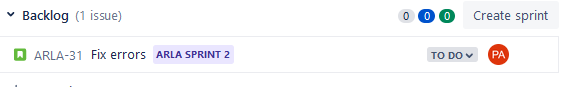
\includegraphics{img/Backlog.png}
    \caption{BackLog}
    \label{fig:my_label}
\end{figure}
The backlog was where any tasks that were incomplete in the sprint were held. It was easy to access and see what is holding the project progress up and who has been assigned the task. 

\subsection{Board}
\begin{figure}[h]
    \centering
    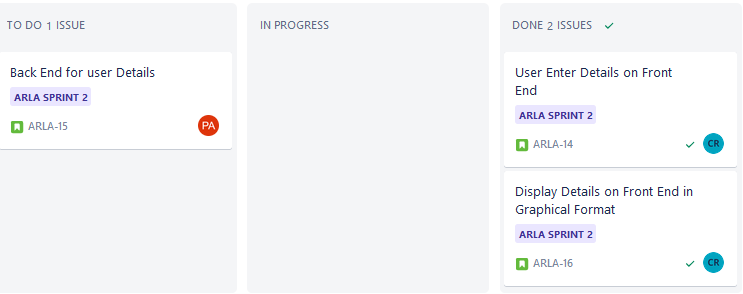
\includegraphics[width=15cm, height=6cm]{img/Board.png}
    \caption{Board}
    \label{fig:my_label}
\end{figure}
The board is a cool feature that basically has 3 categories as seen above. It categorises what needs to be done, what is in progress and what has been completed. Once all tasks have been completed the sprint can be completed and the next sprint will begin. 

\section{Sprints}
Tasks were separated into sprints. There was an idea to have three sprints. Getting each sprint done and moving on to the next sprint was ideal, however there was also flexibility. Should a task or feature take longer than expected, it was agreeable that sprints could be adjusted accordingly, or the task could be moved into the new sprint. 

\subsection{Sprint 1}
It was decided that during sprint 1 the following would be attempted to be completed:
\begin{itemize}
\item Login page implementation
\item Register page implementation
\end{itemize}


\subsection{Sprint 2}
It was decided that during sprint 2 the following would be attempted to be completed:
\begin{itemize}
\item Home page design
\item Graph pages display
\item Pop up with user info
\end{itemize}

\subsection{Sprint 3}
It was decided that during sprint 3 the following would be attempted to be completed:
\begin{itemize}
\item Home page dynamically display data
\item Messaging application
\end{itemize}
The sprints were adjusted as the project progressed, but this was how it was planned originally. 

\section{Research}
After a plan had been organised, the next step was vital. It was important to research the technologies that were going to be used in the development of the web application. Some of the research that was conducted was to do with Neo4J and how to use it as this was going to be a new language that had to be learned. The next bit of research that had to be done was with the graphical side of the application. There are many different tools that can be used to superimpose a graph onto the front end, but it was important to find the best one for this project. Some of these tools researched was D3.js, Neovis and VivaGraphJS among many others. 

\section{Meetings}
Meetings were held on a weekly basis. This was decided on in the early days of the project. The importance of meetings were vital in order to ensure the project was being kept on track and to ensure every team member was doing as much as they could to the best of their ability. The supervisor was a big help in the advice that they gave as well as the reassurance of the work that was done was correct and done to a high standard. Feedback was very important to the progress of the project. 

\section{Project Management Tools }
GitHub was used for the storage and collaboration of the project. This is where any work was stored and continuously updated with any changes and or issues that may have arisen. The commit history was of particular use as there it could be seen what stage the project was at and if an error needed fixing. OneNote from Microsoft was used for documenting any progress or issues as well as minute meetings throughout the duration of the project. The other tool for project management was Jira which was discussed in detail above. 

\chapter{Technology Review}

\section{Intro}

Before any action was taken on what the technologies that were to be used were going to be, a great amount of research needed to be conducted into what would be the most suitable technologies for this project. After much research into many different technologies, it was decided which were suitable and which technologies were not. A further look into why certain technologies were used and why some technologies were initially going to be used but an alternative was instead chosen in the middle of development. \\

\section{Technologies Researched}

Research was a vital part of the development of the application. A poorly researched project could lead to slow development, constant issues that can be avoided easily and just overall is a poor way to conduct the project. Much of the technologies that were researched at the beginning of the project was a suitable choice for this application and lead to a fun development of said application. The first aspect of research on the front end was to what framework and language to use. \\

\section{Language and Framework}

The first part of research was to decide what would be the framework and language that the application would be written in. The decision was initially narrowed down to JavaScript as the language of preference. The reason for the use of JavaScript as the front-end language was due to the fact that JavaScript is widely popular and very commonly used to create interactive web-based applications.\cite{Javascript} JavaScript was very suitable for this application as its main functionality is to allow for users to interact with the application. \\

With that being resolved fairly rapidly, the next decision to be made was to do with the framework that would be used with JavaScript. This was narrowed down to 2 options, React and Angular. There was a personal preference that React be the framework used, however, much research needed to be conducted to see if this was the best suit for the application or if Angular would offer more benefits in the long run. First of all, what are each of these. \\

\subsection{React}

React is an open-source library in JavaScript that is mainly used as a tool for front end development. It is mainly used in building a user interface. It can be used to create single page applications which allow for great efficiency and accessibility.\cite{AngularvsReact}\\

\subsection{Angular}

Angular is a development platform that is built on typescript. One of the issues with Angular that was the learning curve is far steeper than that of React. With the learning curve that will be discussed further down the line in D3.js and other areas as well as the preference for React over Angular, it was decided that React.js was a much better framework for the application.\cite{AngularvsReact} \\

\section{Graph}

There was a huge amount of research needed into the graph side of the application. This was a totally new experience and to ensure that the highest quality graph was being produced while also being flexible to add to, much research was undertaken. There were a number of different technologies that were considered for the project which involved a lot of reading of documentation. These were D3.js, Neovis.js, react-graph-vis and Vis.js. \\

\subsection{Neovis.js}

Neovis.js was one of the technologies that was researched. It is a tool that is used to create graph visualisations on the front end of the application\cite{Neovis}. Neovis was initially the technology that was implemented within the project due to how it is specifically for superimposing graphs from the back end to the front end of applications. However, there was an issue with this in development that led to it being scrapped. The issue was to do with the connection between the database and the front end. There was a constant connection issue to do with web sockets. Many an hour was spent trying to debug and fix but to no avail. Cause of this it was decided that something else would be better to use.\cite{Neovis2}\\

\subsection{react-graph-vis}

Another technology that was researched was react-graph-vis. React-graph-vis was a very intriguing prospect to incorporate into the application. It is another component that allows for displaying network graphs onto the front end of an application. This was another technology that an attempt was made at implementation but again had serious connection issues which made it unfeasible to implement in this project.\cite{React-Graph-Vis} \\

\subsection{Vis.js}

The final technology that was researched but wasn’t used is Vis.js. Another graph visualisation library that has many benefits, but this library did not entirely suit the application. In terms of connection, again there were too many issues, as well as an inability to access the data.\cite{Vis.js} \\

These technologies are very good, but it just did not work with the application that was being designed and implemented here. So it was decided that D3 would be the graph visualiser that would be implemented. \\

\subsection{D3.js}

D3.js was the first technology that was researched. D3 is a JavaScript library which is used for manipulating documents based on data. It allows for the developer to be able to represent data using visualisation.\cite{D3.js} D3.js is an excellent library as it provides a lot of flexibility when it comes to drawing the graph, however it was not as simple to use as other technologies were. However, it was decided that this was the best to use as it allowed for the expansion of the graph pages and to add more interactivity between the application and the user. \\

\section{Node.js}

Node.js is an asynchronous event-driven JavaScript runtime environment that is used as a server-side architecture. Node.js is a good tool to use in developing applications as it is designed to be scalable.\cite{Node.js}\\

Node is an environment that allows for multiple connections to occur at the same time to a server and also is useful when it comes to processing multiple requests at the same time. Node.js is a well run open-sourced tool which upon a connection, a call back is fired and when there is no more work to be done on Node.js’s end, it will go to sleep so to speak.\cite{Node.js}\\ 

\section{Neo4J AuraDB}

Neo4J is the database that was used for the application. There was much deliberation over which would be the best database to use for the application. The idea was to use a no SQL style database so that the user was not in any way fixed in how much information they had to add to the database. Considering the graph aspect of the application, it was decided that Neo4J would be the best suited database due to its use of graphs. Neo4J is a database that stores and manages data in a way that maintains the relationships that are created. \cite{Neo4J}\\

With this now set in motion, the use of Neo4J’s cloud database AuraDB. AuraDB is a fast, reliable, scalable and extremely accessible graph database that is provided as a cloud service. Most importantly as well, AuraDB is secure allowing for information to be stored in a safe environment.\cite{Neo4J2}\\

The non-relational database was crucial to the project as it meant as the applications userbase grew, with more and more data being added, the database could cope with all of this.\cite{Neo4J3}\\

\section{Libraries}

A number of different, npm packages, libraries and other tools were used in the development of this application to provide some extra features and functionality as well as to enhance the user interface as well as the applications functionality. The Libraries that were used required quite an extensive bit of research before implementation to ensure that the best use of them were in place. \\

\subsection{Axios}

Axios was one of the libraries that was used in the development of the application. Axios is a library that serves to create HTTP requests that present externally.  The reason for using Axios is because of how difficult it can be to fetch data from external sources without it. Axios helps in retrieving data and adds it to the state within the application.\cite{Axios} \\

Axios works incredibly well with node.js, in fact its mainly designed to primarily work with node.js. The front end of the application sends HTTP requests to the back end of the application. Axios allows for the retrieval of information and return information to the user. It also allowed the application, to update, and create information. \\

\subsection{React-chat-engine and ChatEngine.io}

Just a quick note that the messenger part of the application was meant to be developed between the front end and the backend. Due to the issues that arose with the backend of the application in the middle of development, it was decided to become a front end only application and to make use of Chatengine.io and firebase. \\

React-chat-engine is a free serverless chat API. It works in conjunction with ChatEngine.io. React-chat-engine is a very useful library that is unique to react. All that is needed is to, as mentioned, work with chatengine.io, and have a public key as well as username and user secret. Chatengine.io provides a Rest API to host chats.\cite{Chatengine}\\

\subsection{Firebase}

Firebase is used in conjunction with react-chat-engine and chatengine.io. Firebase is a platform that is developed by google. It is a backend software that allows for the development of web applications as well as Android and iOS applications. This was used in the application as a way of storing the users that are registered to use the Arla messenger. Again, along with chatengine.io, due to unforeseen circumstances with the backend development, it was anticipated that Firebase would not have been used, but it was a welcome help in the development and success of the final project.\cite{Firebase} \\

\subsection{Bootstrap}

React bootstrap is a unique front end framework to react that is used in the creation and styling of components which is used to create an easy to use and stylish user interface on a web application.\cite{Bootstrap} \\

\subsection{Prop-types}

Prop types was used in the aid of creating the popup that can be seen on the graph pages of the application. The prop-types library is very reusable and can be used to implement a number of different features in an application. Prop-types is used to document the intended types of properties passed to components. React then checks the props passed to components.\cite{prop-types}\\

\subsection{React-google-login}

React-google-login is a react library that makes adding a google login component to a react web application extremely efficient and simple to implement. Google login takes the credentials of a user’s Gmail account which then can be used to store the login credentials and said details can be posted to the back end of the application and allow the server to deal with it. As well as a login system, the react-google-login library allows for the simple implementation of a logout button also. Both of these can be seen implemented in the application.\cite{react-google-login} \\

\subsection{React-router-dom}

The library react-router-dom is a npm package that allows for the implementation of dynamic routing in a web application. It is essentially the navigation aspect of the application. The library, that is unique to react, is very useful when it comes to building single page applications in particular. The library allows for fast navigation throughout the web application, increasing the performance of the application and enhancing the experience for the user.\cite{Router-dom}\\

\subsection{React – select}

React-select is an intriguing library that was made use of in the development of the application. React-select is essentially making use of a dropdown box or select box, but with dynamic data. The great thing about it is that it can be reused in multiple places throughout the project. This was a great use and addition to the application.\cite{Select} \\

\subsection{React – select-country-list}

React-select-country-list is almost like an addition to the react-select library that was mentioned previously. It makes use of the select bar that react select creates, but instead of having to add each country in the world to a list of data and connecting that to the select bar, react-select-country-list does it all for you. This is a very useful library that can be used in lots of different types of applications.\cite{select-country}\\

\subsection{Reactjs-popup}

Reactjs-popup is a react library that creates a simple but effective popup component that is displayed on the click of a button.\cite{popup}\\

\section{Google cloud console}

Google cloud console for this project works in conjunction with the google login library as previously mentioned. The console is a place in which the users, that are accessing the app by logging in or signing up, information linked to their Gmail account is processed and stored. It is how the application identifies a user, checks the users’ details using the credentials and allows for the user to sign in or not. Every user that uses google to sign up has their information stored in a project on the google cloud console.\cite{cloud} \\

\section{Heroku}

Heroku is a cloud platform which allows for the hosting of web applications. On Heroku, a web application can be built, delivered monitored and scaled. It is a very useful service that aids in getting the web application from localhost to the general public. Getting the web application onto Heroku is very simple and only takes a matter of minutes.\cite{Heroku1} \\

The platform is a form of PaaS which is extremely efficient and easy to use. It is a great way to publish a web application without worrying about servers and hardware.\cite{Heroku2} \\

\chapter{System Design}

\section{Design}
The application was made using the React framework. React is a web application framework that is used for creating interactive user interfaces. In addition to the React framework, the graphical designs that were used to superimpose the graph from the Neo4J database was done using D3.js. The first step of the design was to plan it, as previously mentioned in the methodology section. Below are the sample designs that were drawn out and used as a basis for developing the front end of the application. \\

It will be seen from the implementation of the project that the designs are not exactly the same. Some pages were changed with more additional changes added. Below there will be an in depth look at each of the pages on the application and there will be some noticeable differences from the design, but these differences are an improvement to the overall design of the application. \\

\begin{figure}[p]
    \centering
    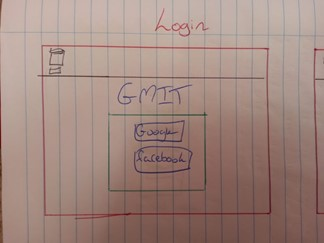
\includegraphics{img/Home Design.jpg}
    \caption{Login Page}
    \label{fig:my_label}
\end{figure}
\\
\begin{figure}[p]
    \centering
    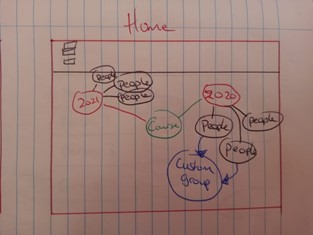
\includegraphics{img/Login.jpg}
    \caption{Home Page}
    \label{fig:my_label}
\end{figure}
\\
\begin{figure}[p]
    \centering
    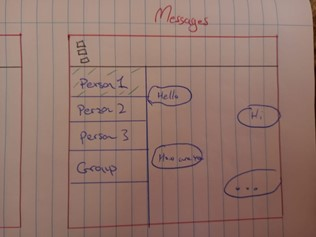
\includegraphics{img/Messenger.jpg}
    \caption{Messenger Page}
    \label{fig:my_label}
\end{figure}
\begin{figure}[p]
    \centering
    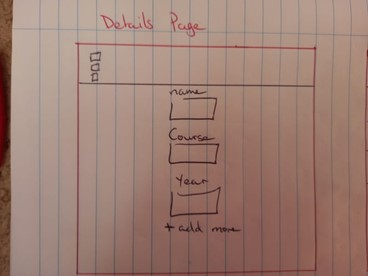
\includegraphics{img/Register.jpg}
    \caption{Register Page}
    \label{fig:my_label}
\end{figure}
\clearpage


\section{Login Page}
The login page was the first point of design that was implemented on the front end of the application. This is the component that the user first sees as they access the website. The page has a design of the GMIT logo at the top on a blue background. There is a google login button to which the user can login to the application. A welcome message is included on the card. The user must login to the website using google. If they do not they will not be able to access the rest of the application as it is protected using protected routes. \\

\subsection{Protected Routes}
Below is an example of the Protected route in action. The user will not be able to access the components that are under the Protected route bracket unless they have successfully logged in. \\
\begin{figure}[h]
    \centering
    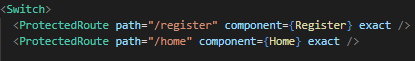
\includegraphics{img/protectedRoute.png}
    \caption{Protected Routes}
    \label{fig:my_label}
\end{figure}

The user must be authenticated. If the user provides valid details, the auth function is set to true. When the user logs out, the Boolean value is set to false. The getAuth function gets the state of the Boolean.
\\
\begin{figure}[H]
    \centering
    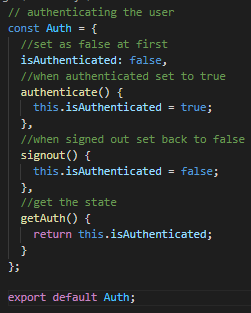
\includegraphics{img/Auth.png}
    \caption{Protected Routes}
    \label{fig:my_label}
\end{figure}

A protected route component is set up. In this function the authentication value from getAuth is retrieved. If the user is authenticated then access to the site is allowed, otherwise, the user is redirected to the login page.\\
\begin{figure}[H]
    \centering
    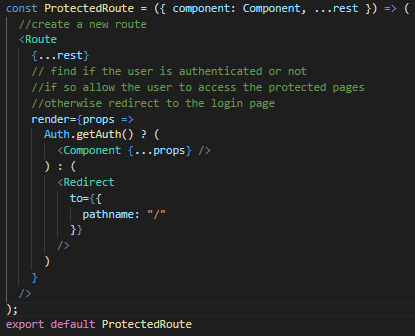
\includegraphics{img/Protected.png}
    \caption{Protected Routes}
    \label{fig:my_label}
\end{figure}

\subsection{Login Page Functionality}
The login page makes use of the react google login library. In this component there is a client id, which is related to the google cloud console. An onSuccess and an onFailure method. \\
\begin{figure}[H]
    \centering
    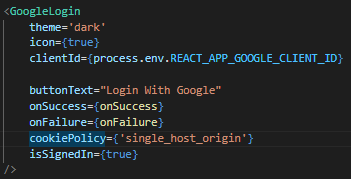
\includegraphics{img/GoogleLogin.png}
    \caption{Google Login}
    \label{fig:my_label}
\end{figure}

The onSuccess method is basically everything that occurs when a user has valid credentials and the login is working correctly. An object is set up that is called googleresponse. This object contains the name, email, id and image URL of the user. The auth method is then called and set to true. The details are then posted to the backend using an axios post method. In order for the user to be able to access the website and to have dynamic data set up for every user, information is set using session storage. This will be elaborated on further in the home page design description. The onFailure method is just a simple message that is printed to the console. \\
\begin{figure}[H]
    \centering
    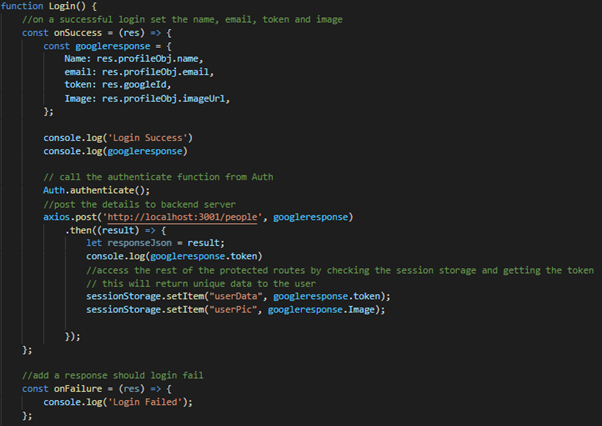
\includegraphics{img/Login1.png}
    \caption{Login}
    \label{fig:my_label}
\end{figure}

Finally, below is a screenshot of the login page in both browser and mobile format.\\
\begin{figure}[H]
    \centering
    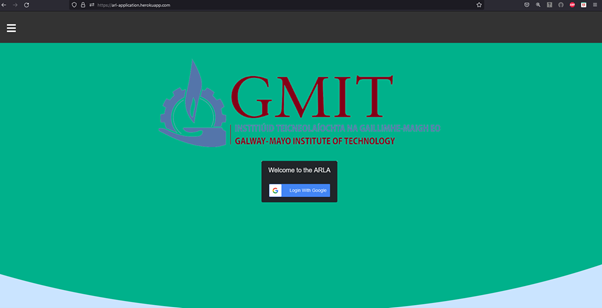
\includegraphics{img/Login2.png}
    \caption{Login}
    \label{fig:my_label}
\end{figure}

\begin{figure}[H]
    \centering
    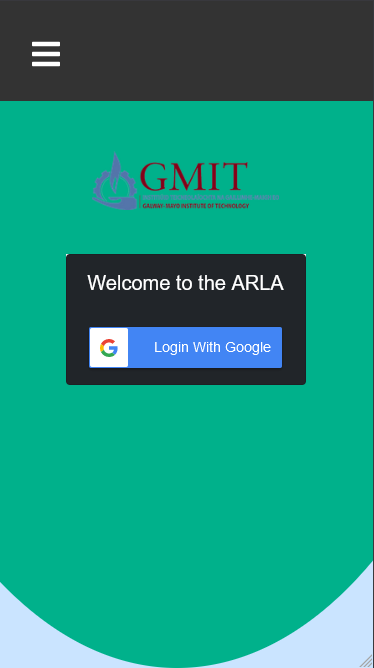
\includegraphics{img/Login3.png}
    \caption{Login}
    \label{fig:my_label}
\end{figure}

\section{Home Page}
The home page is essentially the landing page of the application. This is where the user, after logging in will be redirected to. The home page consists of two different designs depending on the platform the user is on. When the user is on a browser such as chrome, the home page consists of a card with the GMIT logo on it. When the user hovers over the card, it will rotate showing the back of the card. Here is where the user that is logged in details will appear. Below is an example of this\\

\begin{figure}[H]
    \centering
    
\includegraphics{img/Home1.png}
    \caption{Before}
    \label{fig:my_label}
\end{figure}

\begin{figure}[H]
    \centering
    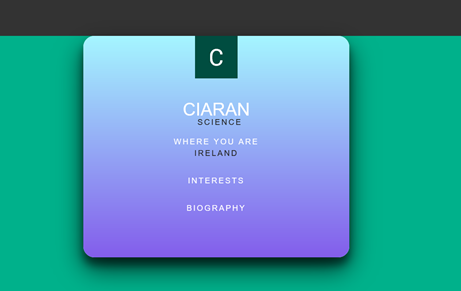
\includegraphics{img/Home2.png}
    \caption{After}
    \label{fig:my_label}
\end{figure}

When the user is accessing the page through a mobile page, there is no card. It is displayed in a simpler format. Below is an example of this. \\
\begin{figure}[H]
    \centering
    
\includegraphics{img/home 3.png}
    \caption{Mobile Platform}
    \label{fig:my_label}
\end{figure}


The home page is where it will display the dynamic and unique information to of the user. It displays the users profile picture, their name, the course they did, where they are now, their interests and finally, hobbies. Session storage is used to get the user that is logged in, it will then use that specific users information to get dynamic data from the back end of the application. This is done using an Axios get request, and that information is displayed to the user. \\
\begin{figure}[H]
    \centering
    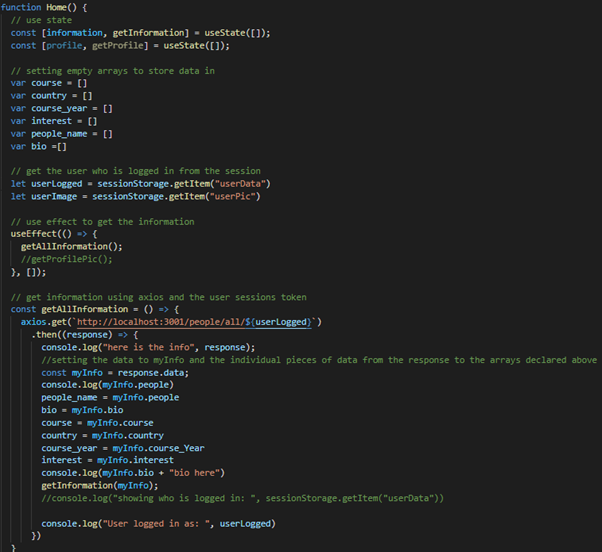
\includegraphics{img/home 4.png}
    \caption{Get Information}
    \label{fig:my_label}
\end{figure}


As seen from the screenshot above, the useStates and empty arrays are set. 2 variables called userLogged and userImage are created. The two respectively are assigned to the session storage userData and session storage userPic. This is how the home page for each user is created dynamically. useEffect is then used to call the getAllInformation method. The getAllIInformation method is where the application connects to the backend of the application and gets all the data from the backend. This is done using an axios get request. Displaying the profile picture is done by using the session storage as mentioned above. The data is retrieved from storage and then displayed in an image style as seen below. \\
\begin{figure}[H]
    \centering
    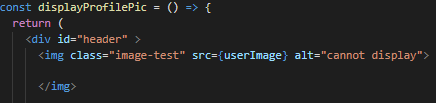
\includegraphics{img/home 5.png}
    \caption{Profile picture}
    \label{fig:my_label}
\end{figure}

The resulting information is then displayed on the card that was shown above if on a web browser. The secondary simpler style is used if on a mobile device. \\
\begin{figure}[H]
    \centering
    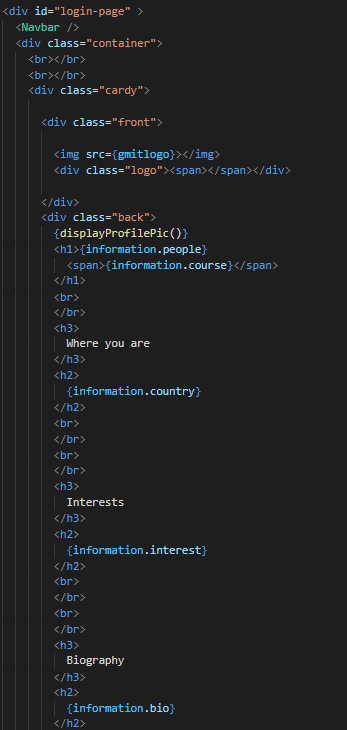
\includegraphics[height=12cm]{img/home 6.png}
    \caption{Display} 
    \label{fig:my_label}
\end{figure}


\section{Register Page}
The register page is where the user can add details to their profile. On the logging in and the creation of the account, the user only has the google login details associated to them. Here is where the user can add their name and biography, course, the year they studied said course, interest and hobbies and where they are now. The user does not have to enter any details here at all, although they will not show up on the home page that has been detailed above. The idea around the application and the use of a no SQL database was to give the user as much flexibility in what they wanted to be shown on their profiles. The register page is divided into 4 cards. The user enters details and clicks on the buttons to add the information to the database. The cards are placed on a carousel, so in order to access the next card, the user must click on next as seen below. \\
\begin{figure}[H]
    \centering
    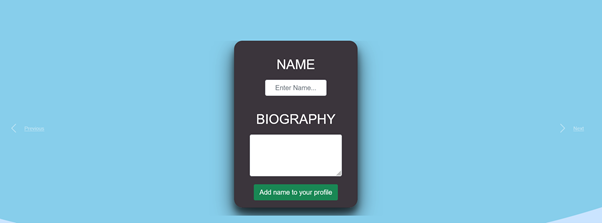
\includegraphics{img/Register1.png}
    \caption{Display} 
    \label{fig:my_label}
\end{figure}

Going to the next item on the carousel will bring up a new card where the user can then add that information to the profile. Once the user is satisfied with the information that is added to the profile, they can then see said information by navigating back to the home page. 
Adding the information and posting it to the backend is done using useState. 
\\
\begin{figure}[H]
    \centering
    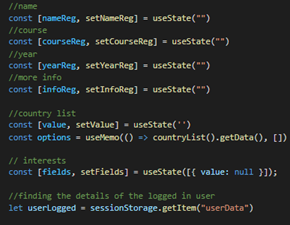
\includegraphics{img/register2.png}
    \caption{States} 
    \label{fig:my_label}
\end{figure}

The addDetails function is created using an axios put request. The reason for this being a put rather than a post will be discussed a little further on in the backend section. This updates the name of the user and the biography of the user. \\

\begin{figure}[H]
    \centering
    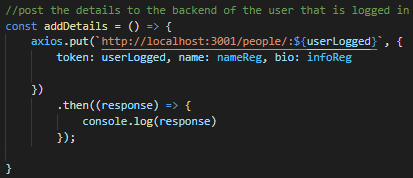
\includegraphics{img/register3.png}
    \caption{Axios} 
    \label{fig:my_label}
\end{figure}

The addCourse function is a post request to the backend and adds the course to the database if not already there. This is also the same for the add country and add interest functions. The add country method however adds the value of the label to the backend. This is because the way a user selects where they are now is by using a react select bar. The add interest method also allows for multiple interests to be passed to the backend of the application. All of these post requests are done by posting the data to the backend as an Object. 
\\
\begin{figure}[H]
    \centering
    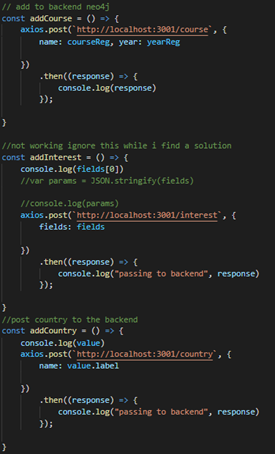
\includegraphics{img/register4.png}
    \caption{Add} 
    \label{fig:my_label}
\end{figure}

The final step of creating a profile is to create links to each object. For example, creating a relationship or link from the user profile to the course. This done by posting the userLogged variable, where information is retrieved from session storage, along with the associated value, i.e. course posts the course value.\\
\begin{figure}[H]
    \centering
    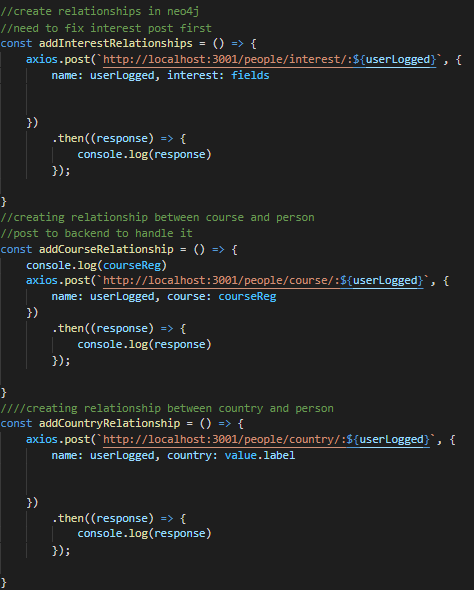
\includegraphics{img/register5.png}
    \caption{Relationships} 
    \label{fig:my_label}
\end{figure}

Below you can also see an example of the card being displayed as a carousel item in code. \\
\begin{figure}[H]
    \centering
    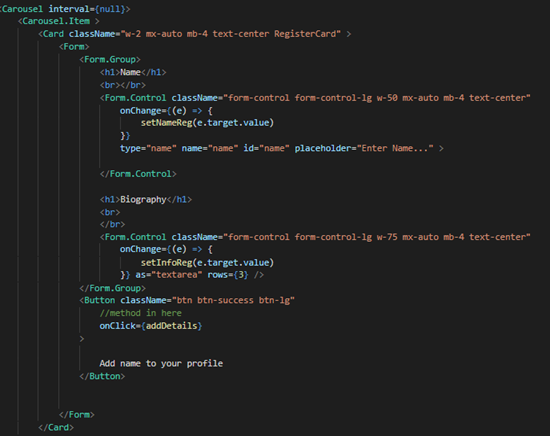
\includegraphics{img/register6.png}
    \caption{Display} 
    \label{fig:my_label}
\end{figure}

The react select bar is created using the react-select-country-list package. It is a useful library that was made use of to create a list of countries rather than individually making the data itself. \\
\begin{figure}[H]
    \centering
    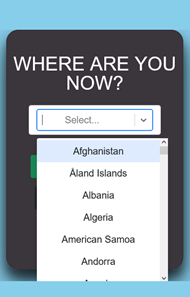
\includegraphics{img/register7.png}
    \caption{Select bar} 
    \label{fig:my_label}
\end{figure}

Adding multiple interests is quite an interesting feature that was also implemented. This allows the user to click a button and it will create a new field where the user can enter another interest. \\
\begin{figure}[H]
    \centering
    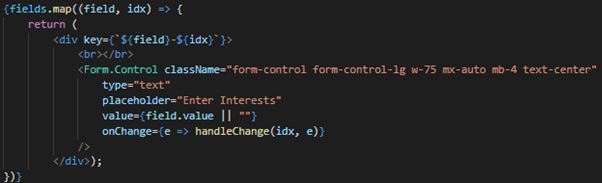
\includegraphics{img/register8.png}
    \caption{Multiple interests} 
    \label{fig:my_label}
\end{figure}
\begin{figure}[H]
    \centering
    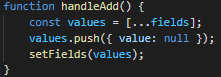
\includegraphics{img/register9.png}
    \caption{Multiple Interests} 
    \label{fig:my_label}
\end{figure}
\begin{figure}[H]
    \centering
    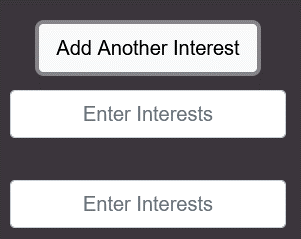
\includegraphics{img/register10.png}
    \caption{Multiple Interests} 
    \label{fig:my_label}
\end{figure}

\section{Graph Page}
The graph page, in essence, is a way of displaying the data from the graph database Neo4J and superimposing it onto the front end of the application for the user to see, use and interact with it. The user is first left with a choice of which course they wish to view the graph of. This is done in similar fashion to the react select bar that was used for countries, this time using the react-select package. After selecting a course, a dynamic page is then loaded with all the information from that specific course being loaded on to the screen. The graph is then drawn with D3.js. The user can interact with the graph where they can click on the user’s name. This will bring up a popup showing the users name and asking if they would like to connect with them in the messenger page. Below is an example of how the graph will look. \\
\begin{figure}[H]
    \centering
    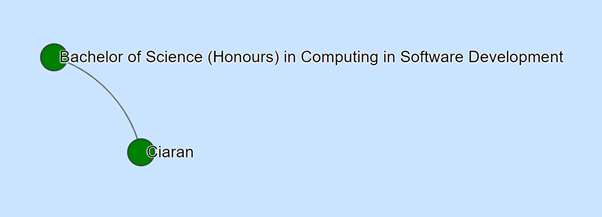
\includegraphics{img/Graph1.png}
    \caption{Graph} 
    \label{fig:my_label}
\end{figure}

As more people register this course and link it to their profile, the more names or nodes will be added to the graph connecting to the main node which is the course name. \\

After much deliberation between the different technologies as mentioned in the Technology Review section, it was decided that D3.js would be the best option to superimpose the graph onto the front end. As well as the issues with the other technologies, those other technologies did not offer the same flexibility that D3.js was offering. D3.js had many benefits outweighing the others, the one issue with it was that it was a very difficult part to learn for the project. \\

An axios get request was used to get all the data for the specific course from the back end of the project. This data is then pushed into an array. 
\\
\begin{figure}[H]
    \centering
    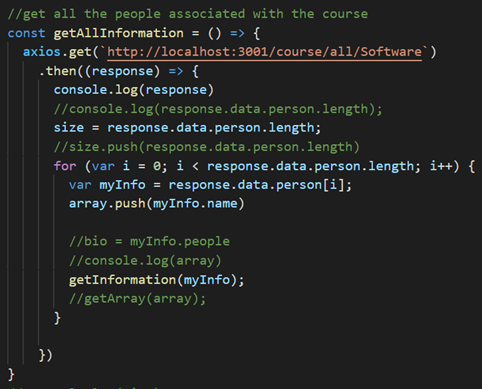
\includegraphics{img/Graph2.png}
    \caption{Get details} 
    \label{fig:my_label}
\end{figure}

The next part is where the D3.js comes into play. The array is looped through to get all the different elements or names that are stored in it from the get request. These are then set as a target for the source. The source and the target are then connected together. \\
\begin{figure}[H]
    \centering
    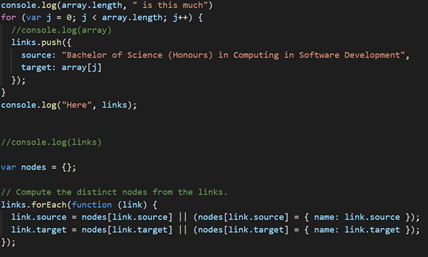
\includegraphics{img/Graph3.png}
    \caption{D3} 
    \label{fig:my_label}
\end{figure}


The next part was to draw the graph itself. First the size of the graph is created and the intricate details such as distance between node and source is created. \\
\begin{figure}[H]
    \centering
    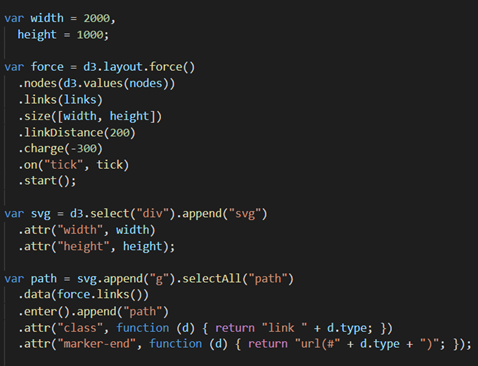
\includegraphics{img/Graph4.png}
    \caption{D3} 
    \label{fig:my_label}
\end{figure}

The variable circle is now drawn and the relevant methods called. The on click method will set the name to appear in the popup and the visibility of the popup will be set to true. The sizing of the text method is also created, this is just simple formatting for any text that appears. \\
\begin{figure}[H]
    \centering
    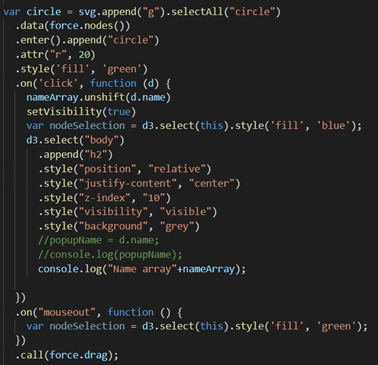
\includegraphics{img/Graph5.png}
    \caption{D3} 
    \label{fig:my_label}
\end{figure}
\begin{figure}[H]
    \centering
    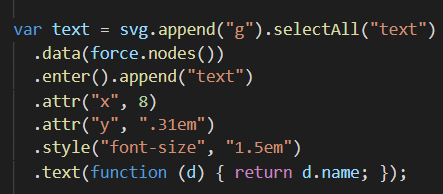
\includegraphics{img/Graph6.png}
    \caption{D3} 
    \label{fig:my_label}
\end{figure}
Finally, the graph is drawn on the target space, the relevant functions are called, and the graph is created successfully. \\
\begin{figure}[H]
    \centering
    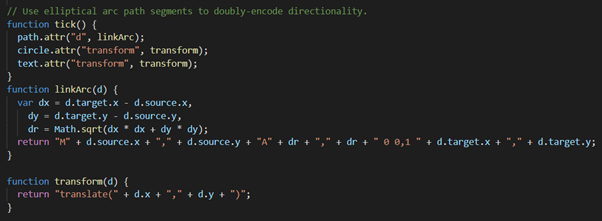
\includegraphics{img/Graph7.png}
    \caption{D3} 
    \label{fig:my_label}
\end{figure}

There are some things that need to be fixed or that can be done to make the graph better or more user friendly which will be discussed in the System Evaluation section. \\

The popup was an intriguing idea that came to mind during one of the meetings with the supervisor. The idea about the popup was that the user can click on a node in the graph, it would display the persons details and have a button which would take the user to the messenger part of the application and they could start a conversation from there. This was done using the package prop-types. \\

The custom popup, again like much of the project, uses useState and useEffect. At the start, the useState is set to false and useEffect is used to update the visibility of the popup.\\
\begin{figure}[H]
    \centering
    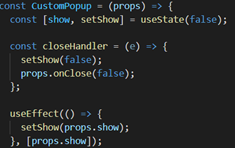
\includegraphics{img/Graph8.png}
    \caption{Popup} 
    \label{fig:my_label}
\end{figure}

The popup then can be used in any part of the application as it was set up as a component, but it was only used on the graph page. The popup contains, the name or title, a close button which links back to the closeHandler function, and the visibility is set to either true or false depending.\\
\begin{figure}[H]
    \centering
    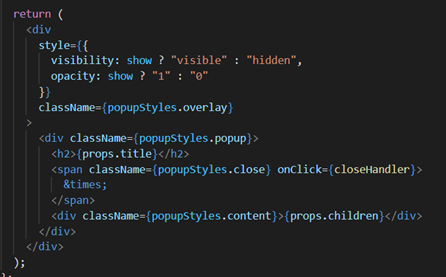
\includegraphics{img/Graph9.png}
    \caption{Popup} 
    \label{fig:my_label}
\end{figure}

\section{Navbar}
The navbar of the application is essentially the user’s tool to navigate the application with ease. Should the user get confused or unsure of where to go, this will be their go to option. The navbar appears in the top left-hand corner of the application, appearing as seen below. \\
\begin{figure}[H]
    \centering
    
\includegraphics{img/nav1.png}
    \caption{Nav icon} 
    \label{fig:my_label}
\end{figure}
Upon clicking this icon, the following navigation bar is displayed onto the screen. \\
\begin{figure}[H]
    \centering
    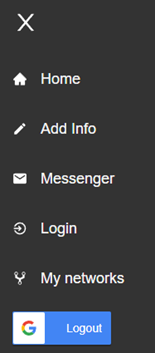
\includegraphics{img/nav2.png}
    \caption{Navbar} 
    \label{fig:my_label}
\end{figure}

The options the user will have to navigate to are as follows: 
\begin{itemize}
\item Home – this redirects the user to the Home Page. 
\item Add Info - this redirects the user to the Register page.  
\item Messenger – this redirects the user to the Messenger page.  
\item Login – redirects the user to the Login Page
\item My Networks – redirects the user to the Graph selection Page 
\item Logout – Logs the user out of the application. 
\end{itemize}

These pages can only be accessed by the user when they have successfully logged in. Sidebar.js is where the navbar is designed. useState once again is set as false at the beginning, as well as setSidebar being set to false. The showSidebar function is set to true when the relevant button is clicked. This so that the navbar does not load onto the screen until clicked. The onSuccess method is what is called when a user has successfully logged out and redirects to the login screen. \\
\begin{figure}[H]
    \centering
    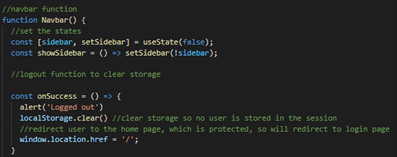
\includegraphics{img/nav3.png}
    \caption{States} 
    \label{fig:my_label}
\end{figure}

When the navbar is selected, the data is then displayed. The items are taken from a page called SidebarData.js. These are displayed in a list with the relevant icon and title. \\
\begin{figure}[H]
    \centering
    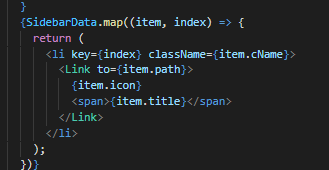
\includegraphics{img/nav4.png}
    \caption{Sidebar} 
    \label{fig:my_label}
\end{figure}

The SidebarData.js script contains a simple const which contains a number of different items. Each one with its own dynamic URL, title and icon. \\
\begin{figure}[H]
    \centering
    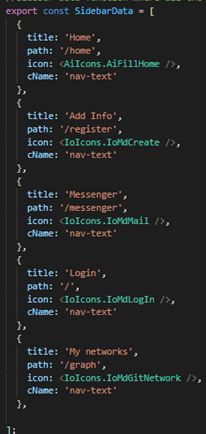
\includegraphics{img/nav5.png}
    \caption{Data} 
    \label{fig:my_label}
\end{figure}

\section{Messenger}

The messenger part of the application allows for users to connect with other registered users. The user can register for the application on the login screen with the ARLA Messenger login. \\
\begin{figure}[H]
    \centering
    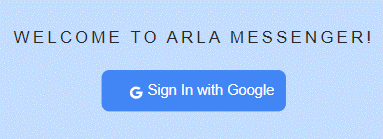
\includegraphics{img/messenger1.png}
    \caption{Login} 
    \label{fig:my_label}
\end{figure}

This will then authenticate the user with firebase. Allowing them to access and use the application. This is done by creating a function called auth using firebase.InitializeApp. This contains an api key, domain, project Id, senderId and appId.  This leads to the AuthContext.js file. This is used to set the user. The user is set to null at first. useEffect is then called into play. Here the auth function from firebase.js is called which then sets the user. The value is then set to user. \\
\begin{figure}[H]
    \centering
    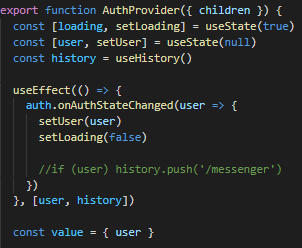
\includegraphics{img/messenger2.png}
    \caption{User} 
    \label{fig:my_label}
\end{figure}

On successful login, the user can then access the messenger part of the application. The user from here can set up new chats, add users to chats, delete chats and most importantly message other users. \\
At this point of the application, chatengine.io comes into play. An axios get request is used to get access to the messenger application. This uses the username and user secret as well as the project ID. Should the user not have logged in correctly they will be redirected to the login screen. \\
\begin{figure}[H]
    \centering
    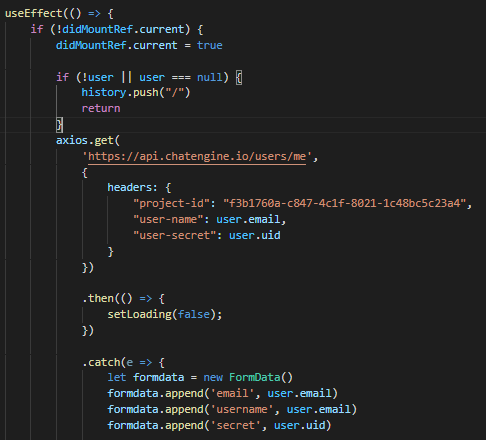
\includegraphics{img/messenger3.png}
    \caption{Get data} 
    \label{fig:my_label}
\end{figure}

Within the catch statement., an axios post request is performed adding a new user to chatengine.io. This is where the private key is posted. 
\begin{figure}[H]
    \centering
    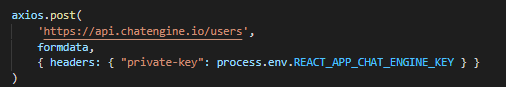
\includegraphics{img/messenger4.png}
    \caption{New user} 
    \label{fig:my_label}
\end{figure}

\section{Backend}

As mentioned previously that there were issues on the backend development of the project, therefore some work that was already there was changed so that it actually connected, interacted and worked with the front end of the application. Some Work was also added to the back end so that the front end could produce a unique home page to the user. These were as follows.

\subsection{Neo4J}
The Neo4J database is stored using AuraDB on the cloud. This is great for security, speed and also for accessibility during the development of the project. The information that was sent from the front end is passed to the back end. The back end, which is done using Node.js, then takes this information and performs queries to store the information in the database and create relationship queries. 
\begin{figure}[H]
    \centering
    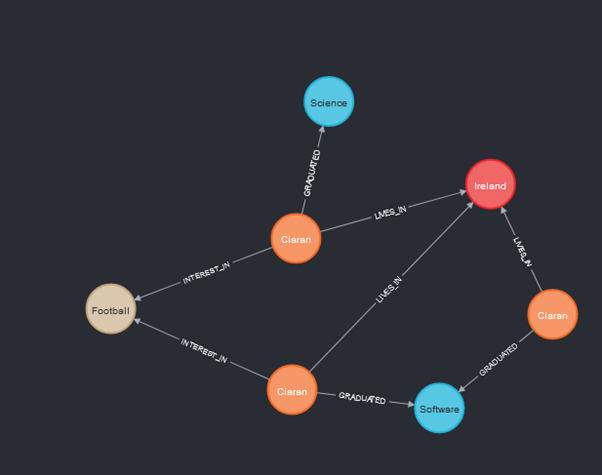
\includegraphics[height=10cm]{img/Backend1.png}
    \caption{Neo4J} 
    \label{fig:my_label}
\end{figure}

Above is a screenshot of the Neo4J database after data has been added by users. The user is created on login with an email and a token being the information that is stored for said user.\\

\begin{figure}[H]
    \centering
    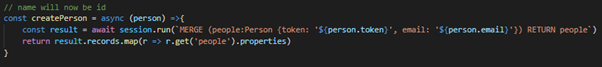
\includegraphics{img/Backend2.png}
    \caption{Create} 
    \label{fig:my_label}
\end{figure}

Once the user accesses the register page and adds their name, an update method is called in which the users name is added to the node that has that associated email. \\

\begin{figure}[H]
    \centering
    \includegraphics{img/backend3.png}
    \caption{Update} 
    \label{fig:my_label}
\end{figure}
\begin{figure}[H]
    \centering
    \includegraphics[width=14cm]{img/backend4.png}
    \caption{Update} 
    \label{fig:my_label}
\end{figure}

Relationships could then be created after information such as course, country and interests were added. This was done using a post method and running a query to create a relationship in the database relating to the information that was passed to the backend.  \\

\begin{figure}[H]
    \centering
    \includegraphics{img/backend5.png}
    \caption{Relationships} 
    \label{fig:my_label}
\end{figure}

\begin{figure}[H]
    \centering
    \includegraphics{img/backend6.png}
    \caption{Relationships} 
    \label{fig:my_label}
\end{figure}

\begin{figure}[H]
    \centering
    \includegraphics{img/backend7.png}
    \caption{Relationships} 
    \label{fig:my_label}
\end{figure}

\begin{figure}[H]
    \centering
    \includegraphics{img/backend8.png}
    \caption{Relationships} 
    \label{fig:my_label}
\end{figure}

\chapter{System Evaluation}

It was very important for the application to be as robust as possible. This was done by testing the application consistently, finding any errors, issues and bugs, ensuring the application was swift in use. It was also important to ensure that the application was simple and easy to use for all users. It was important that the goals set out from the beginning were reached and an evaluation of the system is an important part to check this. There were some aspects of the project that worked extremely well, some were touch and go and some aspects did not work at all. Some insight into all of these will be looked at. 

\section{Robustness}

Before the project was completed, some testing was done using Selenium. Most of the testing done with selenium was basic and did not delve too far into complex testing as during the development of the project, the application was being tested constantly for every possible scenario that could be thought of at the time. During the development there was a constant stream of errors and bugs found. This consistent testing allowed for finding these errors and fixing them before the next stage of development occurred. Long hours of testing were put into the application and even after all that there are still some issues that need to be resolved. Selenium was a helpful tool as it made testing quite a bit faster and easier and also found some blind spots in terms of areas that had not been fully tested.\\

\section{Goals and Objectives}

There are many aspects of the project that matched the goals that were set at the beginning of development. In respect to the goals, the following were achieved successfully or at least partially. In relation to the first goal, the project is successfully hosted on Heroku. The application also is a success in allowing users to connect and message each other. The application is also very easy to use and accessible for all users with varying experience of technology. The application is also very flexible. If the user wants to add no information to their profile, they can do so. This was achieved with the help of the NoSQL database Neo4J. Users can also connect with each other through groups using the messenger part of the application. As many users as they like can be added to the chat. This is a partially completed goal as the mini graph as mentioned in the introduction did not come into being. The project also helped in developing skills in new languages such as Neo4J and D3, as well as improving already known languages such as React.js.\\

\section{Issues}
At the time of submission there are a few errors in which could not be fixed in time. A list of errors, bugs or some things that just needed a bit more work included: 
\begin{itemize}
\item Displaying a list of interests does not incur a space after each interest when displayed on home page. 
\item Carousel not entirely user friendly after all carousel items have been gone through. 
\item Messenger using chatengine.io is not as quick as hoped.
\item Logging into messenger can be a small bit flimsy or slow. 
\item Graph page draws too many times and not just once. 
\end{itemize}

\section{What Worked}

Overall, the quality and efficiency of the project is to a high standard with goals met. There are many aspects of the application that were integrated to the project well and add great worth to the quality of the product. Some of the things that worked extremely well and will be useful for any further work on this application or that can be used on new projects are the navbar, the login system, the home page, the register page, the messenger page and parts of the graph page. \\

\subsection{Navbar}

The Navbar is a part of the application that is fully functional and of high quality that is also very reusable for future applications. The Navbar is a useful tool for the user of the application as it is a constant throughout the project and can be used to navigate the user home should they get overwhelmed or lost in the application. \\

\subsection{Login}

The login system is another part of the application that is of high quality. The npm package react-google-login is of high efficiency and made the development of the login system simple and effective. This is another part of the application that can be used in any other project that would require a login system. \\

\subsection{Home}

The home page is an efficient and simple design with dynamic information depending on the user that is logged in. It is efficient and styled using CSS to change its style depending on the device the application is run from. Data is successfully collected from the backend using axios at great efficiency. \\

\subsection{Register}

The register page is fully functional and of good quality. The axios post request that is used to send data to the backend is quick and efficient, allowing users to add however much information they like to their profile. There is one aspect needs some work on that will be discussed further below.\\

\subsection{Messenger}

The messenger page does exactly what it needs to do, allow users of the application to message each other. The messaging system using chatengine.io is of decent quality and a very interesting aspect of the application in terms of development. \\

\subsection{Graph}

The graph page is perhaps the most interesting and most appealing part of the application and a unique selling point of an application like this. There is a dynamic graph for each subject, displaying all the names of people who have linked to a course. D3 was an excellent help in drawing the graphs and probably the best technology to use as it allowed for the popup to be developed for each individual node. Something the other technologies researched like Neovis.js would not allow. \\

\section{What Can Be Improved}

Along with the parts of the application that worked very well there are some areas that need work or did not gel well with the application created. Some of these are aspects of the graph page, the overall efficiency of the messenger application and the carousel item. Also, due to the issues that occurred during development, the backend is not entirely optimal. \\

\subsection{Graph}

One of the issues that came across in development with the graph page was that the graph kept drawing multiple times. The graph would draw every time a node was accessed from the get request. For example, if there were 5 nodes in total in the graph, the graph then drew at least 5 times. With a bit more time and a bit more of an understanding of D3.js, this problem is very fixable. \\

\subsection{Messenger}

As much as the messenger aspect of the application worked well overall with the application, there was one issue that was blatantly obvious. It is not efficient; it is very slow. This can be seen at first when logging in. After logging in with google in the first part of the application, if the user tries to login to the messenger, they need to give the browser a few seconds before they attempt it otherwise an error will occur, and the user can’t login. The next issue with efficiency was to do with the sending and receiving of messages. It could sometimes be very slow to send, some messages would send twice and then there were issues with connecting now and again. Chatengine.io is just not really optimal and especially not a good choice of technology for a large-scale project with lots of users. Issues with the backend development in the project did not help this aspect of the project. With more time, the messenger page could be made far more efficient. \\


\subsection{Register Page: Carousel}

The carousel item is not really a huge issue more of a minor design issue. When the user adds information and clicks the buttons on each card, at the very end after the last card when the user clicks on next, the last card item stays on the screen until the carousel items have been looped through. A small issue, but certainly something that can be improved upon. \\

\chapter{Conclusion}

Overall, the project was a success. There were so many aspects of the project that went well. The project in the end reached many of the goals that were set and reached many that were seen as a goal that may not be achievable in the time frame. A great deal was learned about so many different aspects of the project such as planning and methodology, research into new technologies and learning more about known technologies, development and testing. As well as this, there was a lot learned about how any projects that are carried out in the future can be improved based on the experience of this project. As well as this, a lot of soft skills such as communication skills were greatly improved upon. \\

\section{Goals Achieved}
In terms of the goals that were talked about in the introduction, the project was a success in meeting these.  The goals that were achieved, whether a complete success or partial success, were as follows:
\begin{itemize}
\item Creating a fully responsive web application hosted on Heroku
\item Make the website user friendly
\item Allow user to have free reign when it comes to the amount of detail added to the application
\item Create groups for contacting other users
\item Gain greater understanding of technologies used
\item Create google login system
\item Create dynamic home pages
\item Draw graphs using D3.js
\item Improve soft skills
\item Improve software testing skills
\item Improve skill of using GitHub, Jira, OneNote
\end{itemize}

\section{What was Learned}

A great deal was learned during the planning and the development of this project. Planning and methodology were a huge benefit to the finish product and the ease the burden of pressure during development. This is also a huge benefit for any future projects that take place, as great experience was taken from this project. The project cycle had so many issues to overcome and great experiences to learn from. With all the learning experiences that were obtained, it will highly benefit the future as any similar problems will now be known how to be dealt with properly and efficiently. The use of planning tools such as Jira were a major help and added a great deal to the project cycle. Being able to have a set plan, that is also open to changes as the project progresses was a huge help in planning sprints. Jira is a tool that will certainly be considered if not used in any future developments or projects. \\

\subsection{React.js and D3.js}

A lot of new interesting features were learned during the development of the application. This included the likes of D3.js. It was a very intriguing prospect to learn about the concept of using this to superimpose the graph from the backend on to the front end of the application. Although there is a lot of different things to learn from D3, this was a great way to be introduced to it. D3.js would be a great choice and first choice for any future projects that require a feature that draws on the front end. \\

As well as learning new features like D3, it was important to increase the knowledge of a language that was already experienced, this being React.js. Improving the knowledge of this language and incorporating new and interesting things into the project was an important goal. A lot of interesting things were learned in React.js including the popup that appears on the graph page, using google as a login system, the interactive navigation bar and many more. In terms of improving the knowledge of React.js, the project was a complete success in those terms. \\

\subsection{Neo4J}

Neo4J was another language that was brand new in this project. Getting to learn a new database was important, especially one as intuitive and fascinating as Neo4J. The no SQL style to it made things very easy to get an understanding of what was happening. After much documentation reading, the use of Neo4J is actually quite simple. It was a great learning experience and a database that would be heavily considered in any future projects and developments. \\

\subsection{Research}

The research aspect was an absorbing activity. There was so much information in documentation for the languages, that so many new features were learned, including some that were not needed for this project but will definitely be looked at for future projects. The research was useful for the project, but also has given a drive for future projects, as there are so many different things that could be implemented. \\

\section{Future improvement}

The project cycle was a great learning experience, from all the aspects mentioned above like learning new technologies, improving on skills already obtained and the great experience of planning a project. There are so many different things to take from the project that can improve this and every other project that will be worked upon in the future. In future, a plan will definitely be made with Jira but along with this, a bit more weekly documentation is one aspect that can definitely be improved upon. Weekly documentation is one aspect that could have done a bit more work on. It would have made for greater communication and also it would help to go back and read upon any issues that took place, or to just see what the overall project cycle looked like in hindsight. Future improvements can also definitely take place in the development and coding of the project. One aspect that could be used a little more is the issues section on GitHub. It is a feature that wasn’t used and it is a small regret as it would have been good to experience using the feature, however, it is definitely something that will be taken advantage of in future. \\

\section{Closing}

Overall, the project was a success and was a major source of pride. The project gave great new experiences, showed how skills such as programming improved majorly over the course of the project cycle and importantly was good fun to develop. There were so many different things learned in the planning and development stages of the project. Importantly, the project has given the drive to improve and give any future projects that are developed the platform to reach the next stage and improve them even further. 

\chapter{Appendices}

\subsection{Github source code}
\url{https://github.com/CiaranRoche203/Arla-App-FrontEnd}\\
\url{https://github.com/CiaranRoche203/Arla-App-Backend}\\

\subsection{Heroku Hosted Application}
\url{https://arl-application.herokuapp.com/}\\
